% Exact TikZ reconstruction of the original PointNet surrogate figure.
% Coordinates are the pixel coordinates of the original drawing
% (2576 x 836, y pointing down), so the result overlays the original.
% Build:
%   pdflatex surrogate-architecture.tex
%   pdftoppm -png -r 300 -singlefile surrogate-architecture.pdf ../public/images/projects/surrogate-pointnet-architecture
\documentclass[tikz,border=0pt]{standalone}
\usepackage[T1]{fontenc}
\usepackage{helvet}
\renewcommand{\familydefault}{\sfdefault}
\usetikzlibrary{arrows.meta}

\definecolor{encF}{HTML}{FFF2CC}
\definecolor{decF}{HTML}{E06666}
\definecolor{opF}{HTML}{CFE2F3}
\definecolor{gfF}{HTML}{999999}

\begin{document}
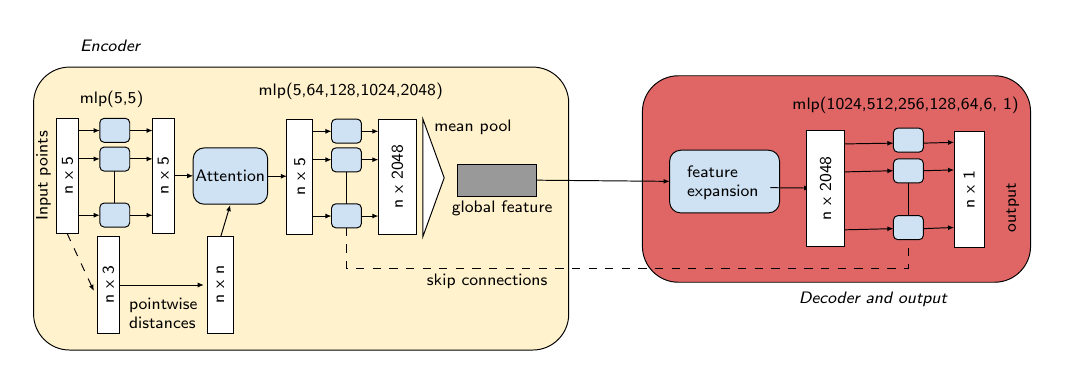
\begin{tikzpicture}[x=0.005cm, y=-0.005cm,
  font=\fontsize{5.8}{6.9}\selectfont,
  line width=0.35pt, >={Latex[length=2.2pt,width=1.8pt]},
  tens/.style={draw, fill=white},
  op/.style={draw, fill=opF, rounded corners=1.6pt},
  lbl/.style={inner sep=0pt},
]
\useasboundingbox (0,0) rectangle (2576,836);

% ---- backgrounds ----
\draw[fill=encF, rounded corners=13pt] (15,100) rectangle (1373,818);
\draw[fill=decF, rounded corners=13pt] (1560,122) rectangle (2545,646);
\node[lbl, font=\fontsize{5.8}{6.9}\selectfont\itshape] at (209,45) {Encoder};
\node[lbl, font=\fontsize{5.8}{6.9}\selectfont\itshape] at (2145,690) {Decoder and output};

% ---- encoder: first shared MLP ----
\node[lbl, rotate=90] at (40,376) {Input points};
\draw[tens] (74,230) rectangle (129,522);   \node[lbl, rotate=90] at (101,376) {n x 5};
\node[lbl] at (213,182) {mlp(5,5)};
\foreach \y in {230,303,445} { \draw[op] (183,\y) rectangle (259,\y+61); }
\draw (221,364) -- (221,445);
\foreach \y in {261,333,476} { \draw[->] (129,\y) -- (183,\y); \draw[->] (259,\y) -- (317,\y); }
\draw[tens] (317,230) rectangle (372,522);  \node[lbl, rotate=90] at (344,376) {n x 5};

% ---- attention ----
\draw[->] (372,376) -- (420,376);
\draw[draw, fill=opF, rounded corners=4pt] (420,305) rectangle (609,448);
\node[lbl] at (514,376) {Attention};
\draw[->] (609,377) -- (658,377);

% ---- encoder: second shared MLP ----
\draw[tens] (658,232) rectangle (722,524);  \node[lbl, rotate=90] at (690,378) {n x 5};
\node[lbl] at (820,162) {mlp(5,64,128,1024,2048)};
\foreach \y in {232,305,447} { \draw[op] (771,\y) rectangle (847,\y+61); }
\draw (809,366) -- (809,447);
\foreach \y in {263,335,478} { \draw[->] (722,\y) -- (771,\y); \draw[->] (847,\y) -- (890,\y); }
\draw[tens] (890,232) rectangle (987,525);  \node[lbl, rotate=90] at (938,378) {n x 2048};

% ---- mean pool and global feature ----
\draw[fill=white] (1003,232) -- (1057,381) -- (1003,530) -- cycle;
\node[lbl] at (1130,253) {mean pool};
\draw[fill=gfF] (1090,347) rectangle (1291,428);
\node[lbl] at (1204,458) {global feature};

% ---- pointwise distances ----
\draw[->, dashed] (100,522) -- (168,668);
\draw[tens] (176,530) rectangle (234,775);  \node[lbl, rotate=90] at (205,652) {n x 3};
\draw[->] (234,653) -- (447,653);
\node[lbl, align=left, anchor=west] at (256,724) {pointwise\\distances};
\draw[tens] (457,530) rectangle (521,775);  \node[lbl, rotate=90] at (489,652) {n x n};
\draw[->] (490,530) -- (514,450);

% ---- skip connections ----
\draw[dashed] (809,508) -- (809,610) -- (2235,610) -- (2235,538);
\node[lbl] at (1166,643) {skip connections};

% ---- decoder ----
\draw[->] (1291,387) -- (1629,390);
\draw[draw, fill=opF, rounded corners=4pt] (1629,311) rectangle (1908,470);
\node[lbl, align=left, anchor=west] at (1672,393) {feature\\expansion};
\draw[->] (1885,406) -- (1986,407);
\draw[tens] (1977,262) rectangle (2073,554); \node[lbl, rotate=90] at (2025,408) {n x 2048};
\node[lbl] at (2228,198) {mlp(1024,512,256,128,64,6, 1)};
\foreach \y in {255,333,477} { \draw[op] (2197,\y) rectangle (2273,\y+61); }
\draw (2235,394) -- (2235,477);
\foreach \ya/\yb in {295/293, 366/363, 513/510} { \draw[->] (2073,\ya) -- (2197,\yb); }
\foreach \ya/\yb in {293/291, 363/361, 510/507} { \draw[->] (2273,\ya) -- (2351,\yb); }
\draw[tens] (2351,264) rectangle (2427,557); \node[lbl, rotate=90] at (2389,410) {n x 1};
\node[lbl, rotate=90] at (2500,457) {output};
\end{tikzpicture}
\end{document}
